\documentclass[12pt,answers]{exam}

\usepackage{amsmath,amsfonts,amssymb,mathtools,physics,commath}
\usepackage{todonotes}
\usepackage{float}
\usepackage{multicol}
\usepackage{fancybox}
\usepackage{siunitx}
\usepackage{cancel}

\newcommand{\inv}{^{-1}}
\newcommand{\RR}{\mathbb{R}}

\pagestyle{headandfoot}
\firstpageheadrule
\runningheadrule
\firstpageheader{Math 221}{Exam 2|Solutions, Page \thepage\ of \numpages}{2017 Summer}
\runningheader{Math 221}{Exam 2|Solutions, Page \thepage\ of \numpages}{2017 Summer}
\runningfooter{}{}{}

\begin{document}
% \maketitle
\begin{questions}

\question
\begin{parts}
\part[6]
Draw the region bounded by the curves.
Then, use the disk method to find the volume when the region is rotated around the $x$-axis.
\[
    f(x) = \sqrt x, \quad x = 0, \quad x= 4 \qand y=0.
\]
\begin{solution}
\begin{figure}[H]
    \centering
    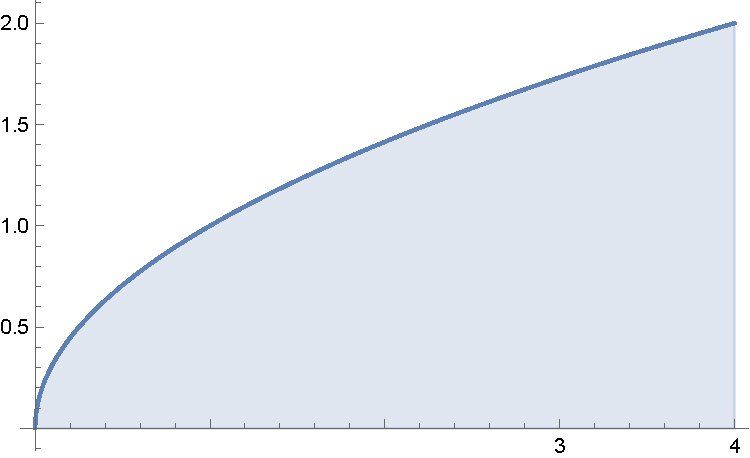
\includegraphics[width=.4\linewidth]{graphics/2017-summer-1-sol.pdf}
\end{figure}
\begin{align*}
    V = \pi \int_0^4 (f(x))^2 \dif x
    = \pi \int_0^4 x \dif x
    = \pi \eval{\frac{x^2}{2}}_0^4 = \boxed{8\pi}
\end{align*}
\end{solution}

\part[6]
Use shell method to find the volume generated when the region between the curves
\[
    y=\sqrt{x},\quad y=x^2 \quad \text{rotated around y-axis}
\]
\begin{solution}
    These curves intersect at $x=0, 1$.
    The volume is thus
    \begin{align*}
        V 
        &= \int_0^1 x (\sqrt x - x^2) \dif x
        = \int_0^1 x^{3/2} - x^3 \dif x \\
        &= \eval{\frac 25 x^{5/2} - \frac 14 x^4}_0^1 
        = \frac 25 - \frac 14 
        = \boxed{\frac{3}{20}}
    \end{align*}
\end{solution}

\end{parts}

\newpage
\question
\begin{parts}
\part[6]
Find the arclength of the function $f(x) = \frac 43 x^{3/2}$ where $0 \le x \le 1$.
\begin{solution}
\begin{align*}
    f'     & = \frac 43 \cdot \frac 32 x^{1/2} = 2 x^{1/2} \\
    (f')^2 & = 4x                                          \\
    L      & = \int_0^1 \sqrt{1+(f')^2} \dif x             \\
           & = \int_0^1 \sqrt{1+4x} \dif x                 \\
           & = \eval{\frac14 \frac 23 (1+4x)^{3/2}}_0^1    \\
           & = \boxed{\frac 16 (5^{3/2} - 1)}
\end{align*}
\end{solution}

\part[6]
Find the surface area of the volume generated by revolving the curve $y=x^2$ from $(1,1)$ to $(3,9)$ around the $y$-axis.
\begin{solution}
    \begin{align*}
        SA &= \int 2\pi x \dif s \\
        &= \int_1^3 2\pi x \sqrt{1+ \left(\dod{y}{x}\right)^2} \dif x \\
        &= \int_1^3 2\pi x \sqrt{1+ 4x^2} \dif x \qquad (u = 1+4x^2; \dif u = 8x\dif x)\\
        &= \frac\pi4 \int_5^{37} \sqrt{u} \dif u \\
        &= \frac\pi4 \frac 23 \eval{u^{3/2}}_{5}^{37} \\
        &= \boxed{\frac\pi6 (37^{3/2} - 5^{3/2})} 
    \end{align*}
\end{solution}
\end{parts}

\newpage
\question[12]
Find the work required to pump all the water out of a cylinder that has a circular base of radius 5 ft and height 200 ft. Use the fact that the density of water is 62 lb/ft$^3$.
\begin{solution}
    \begin{align*}
        \text{force} &= \text{vol} \cdot \text{density} \\ 
        &= 25\pi \dif y \cdot 62 \\ 
        \text{Work} &= \int \text{force} \cdot \text{distance} \\ 
        &= \int_0^{200} 25 \pi \cdot 62 \cdot (200-y) \dif y \\ 
        &= 62 (25) \pi \left[ 200y - \frac{y^2}{2}\right]_0^{200} \\ 
        &= 62 (25) \pi \left[ 200^2 - \frac{200^2}{2}\right] \\ 
        &= 62 (25) \pi \left[ \frac{200^2}{2}\right] \\ 
        &= 31(25) \pi \cdot 200^2\ \text{lb}\cdot\text{ft}
        = \boxed{31\,000\,000\pi\ \text{lb}\cdot\text{ft}}
    \end{align*}
\end{solution}

\newpage
\question[12]
Let $R$ be the region bounded above by the graph of the function $f(x) = x^3$ and below by the $x$-axis from $x=0$ to $x=3$. 
Find the centroid of the region.
\begin{solution}
    \begin{align*}
        M &= \int_0^3 x^3 \dif x 
        = \eval{\frac{x^4}{4}}_0^3 
        = \frac{81}{4} \\ 
        M_x &= \frac12 \int_0^3 (x^3)^2 \dif x 
        = \frac12 \eval{\frac{x^7}{7}}_0^3
        = \frac{3^7}{14} \\ 
        M_y &= \int_0^3 x \cdot x^3 \dif x 
        = \eval{\frac{x^5}{5}}_0^3 
        = \frac{3^5}{5} \\
        \overline x &= \frac{M_y}{M} 
        = \frac{3^5}{5} \cdot \frac{4}{3^4} = \frac{12}{5} \\
        \overline y &= \frac{M_x}{M} 
        = \frac{3^7}{14} \cdot \frac{4}{3^4} = \frac{54}{7}
    \end{align*}
    The centroid is $\boxed{\left(\frac{12}{5}, \frac{54}{7}\right)}$
\end{solution}

\newpage
\question
\begin{parts}
\part[6]
Find the derivative $\dod{}{x} (\tanh\inv x)^2$.
\begin{solution}
    $2 \tanh\inv x \cdot \dfrac{1}{1-x^2}$
\end{solution}

\part[6]
Determine the limit of the sequence or show that the sequence diverges. 
If it converges, find its limit.
\[a_n = \left(1-\frac 2n\right)^n\]
\begin{solution}
    Letting $L = \lim_{n\to\infty} a_n$,
    \begin{align*}
        \ln L 
        = \lim_{n\to\infty} n \ln(1 - \frac 2n)
        &= \lim_{n\to\infty} \frac{\ln(1 - \frac 2n)}{n^{-1}} \\
        &\overset{L'H}{=} \lim_{n\to\infty} \frac{\frac{1}{1 - \frac 2n} \cdot 2n^{-2}}{-n^{-2}} \\
        &= -2 \lim_{n\to\infty} \frac{1}{1-\frac2n} 
        = -2
    \end{align*}
    Therefore $L = \boxed{e^{-2}}$
\end{solution}

\end{parts}

\end{questions}
\end{document}